\documentclass{school-22.101-notes}
\date{November 2, 2011}

\begin{document}
\maketitle

\topic{Application of S-wave: n-p Scattering}
We apply S-wave approximation to n-p scattering in a Finite Square Well with $-V_0$ potential:
\begin{align}
\begin{cases}
u(r) = A \sin(k_1 r) & r \le r_0, k_1 = \frac{\sqrt{2 \mu (E+V_0)}}{\hbar} \\
u(r) = C \sin(k_2 r + \delta_0) & r > r_0, k_2 = \frac{\sqrt{2 \mu E}}{\hbar} 
\end{cases}
\\
\boxed{k_1 \cot (k_1 r_0) = k_2 \cot (k_2 r_0 + \delta_0) } \label{relation}
\begin{cases}
A \sin (k_1 r_0) = C \sin (k_2 r_0 + \delta_0) & u_1(r_0) = u_2(r_0) \\
A k_1 \cos (k_1 r_0) = C k_2 \cos (k_2 r_0 + \delta_0) & u^{\prime}_1 (r_0) = u_2^{\prime} (r_0) 
\end{cases}
\end{align}
Combine the transcendental relation Eq.~\ref{relation}, and the cross section relation Eq.~\ref{sigma} ($B$ means bound state, $E$ is the energy of the neutron, $E_B$ is the binding energy. ):
\begin{align}
k_2 r_0 + \delta_0 &= k_2 r_0 - ak_2 \approx -ak_2 \approx \delta_0 \\
\mathrm{RHS} &= k_2 \cot (k_2 r_0 + \delta_0) \approx k_2 \cot (\delta_0) \\
k_1 \cot (k_1 r_0) &\approx k_1^B \cot (k_1^B r_0) = - k_2^B  = k_2 \cot (\delta_0) \\
\cot (\delta_0) &= -\frac{k_2^B}{k_2} \\
\sin^2 (\delta_0) &= \frac{1}{1 + \cot^2 (\delta_0)} = \frac{1}{1 + \left( \frac{k_2^B}{k_2} \right)^2 } = \frac{k_2^2}{k_2^{B2} + k_2^2} \\
\sigma &= \frac{4\pi}{k_2^2} \sin^2 (\delta_0) = \frac{4\pi}{k_2^2 + \left(k_2^B \right)^2 } = \frac{4\pi \hbar^2}{2 \mu (E + E_B) } \xrightarrow{E \ll E_B} \frac{4 \pi \hbar^2}{2 \mu} \frac{1}{E_B} \\
&\xrightarrow{E_B = 2.22 \mathrm{ MeV}} 2.3 \mbox{ b} 
\end{align}
Notice $\sigma (\theta) = 2.3$ b is significantly smaller than the measured 20 b. The missing piece is the spin-spin coupling component.

\textbf{Spin-spin Coupling}: Recall $S=0$ is singlet with P=1/4, $S=1$ is triplet with P = 3/4. 
\begin{align}
\sigma( \theta) &= \frac{3}{4} \sigma_T (\theta) + \frac{1}{4} \sigma_S (\theta) = \frac{3}{4} \frac{1}{k_2^2} \sin^2 (\theta_{ot} ) + \frac{1}{4} \frac{1}{k_2^2} \sin^2 (\theta_{os} ) \\
\sigma &= 4 \pi \sigma (\theta) = \frac{4 \pi \hbar^2}{2 \mu} \left[ \frac{3}{4} \frac{1}{E_B} + \frac{1}{4} \frac{1}{E^*} \right] 
\end{align}\footnote{we can write $\sigma = 4 \pi \sigma(\theta)$ because l=0 is symmetric potential, so we don't need to integrate here} 
Plug in $E_B = 2.22 \fsp \MeV, E^* = 0.077 \fsp \MeV$, $\sigma = 19$ b, which is a good approximation for 20b. 


Scattering experiments (by Prof. Li on 10/31/12): 
we consider shotting a neutron at a neutron, shotting a proton at a neutron, shotting a proton at a proton: 
\begin{itemize}
\item $\displaystyle a^{\mathrm{singlet}}_{nn} = -16.6 \fm$. 
\item $\displaystyle a^{\mathrm{singlet}}_{pp} = -7.82 \fm$. If we remove the Coulomb effect, $\displaystyle \tilde{a}^{\mathrm{singlet}}_{pp} = -17.1 \fm \sim a^{\mathrm{singlet}}_{nn}$. This is called `charge' symmetry. 
\item $\displaystyle a^{\mathrm{singlet}}_{np} = -23.72 \fm$, which is called `nearly charge' independence. 
\item $\displaystyle a^{\mathrm{triplet}}_{np} = 5.423 \fm$. There is only 1 weakly bound state. 
\end{itemize}

We add three pieces of physics that depends on spins: 
\begin{enumerate}
\item Spin-spin dependency. 
\begin{align}
 \frac{\expect{s_1 \cdot s_2}}{\hbar^2} &= \frac{S^2 - S_1^2 - S_2^2}{2 \hbar^2}  = \frac{S(S+1) - \frac{1}{2} \frac{3}{2} 2 }{2 \hbar^2} = \left\{  \begin{array}{cc} - \frac{3}{4} & S = 0 \\ \frac{1}{4}  & S= 1 \end{array} \right. \\
V &= V_1 (r) \left( \frac{1}{4} - \frac{S_1 \cdot S_2}{\hbar^2} \right) + V_3 (r) \left( \frac{3}{4} + \frac{S_1 \cdot S_2}{\hbar^2} \right)
\end{align}


\item Spin-orbit dependency (velocity dependency). Basically $\displaystyle V_{so}(r) \to V_{so} (r) L \cdot S$. Spin polarizer that breaks the left and right symmetry: there is a concentration effect to the neutrons coming in with up spin to move upwards. 

\item Tensorial-spin dependency (electric quadrapole): from experiments, we observe that deuteron with $I = 1, S=1$ is 96\% s-wave bound state, 4\% d wave ($l=2$). We know that $l=1$ is forbidden from $\pi = (-1)^l = 1^+$, so $l$ can only be even. Then the tensirial force: 
\eqn{ V_T(r) = V \left[ 3 \frac{(S_1 \cdot x) (S_2 \cdot x)}{|x|^2} - S_1 \cdot S_2 \right] }
where the $3 \frac{(S_1 \cdot x) (S_2 \cdot x)}{|x|^2}$ is non-centripetal (because a centripetal force should only be depend on $x^2$) and this term gives the d-wave characteristics.  
\end{enumerate}

[FIXME] insert plot of Singlet and triplet potential vs. r. 
There is an approximate isospin symmetry between a neutron and a proton, that is, if we double swap the position and the spin of a neutron with a proton, we should preserve the symmetry. Given $S=0, \pi = -1$, then $L$ has to be odd, that is, $L=1,3,5$ and $L \neq 0$. Thus the triplet state $V_1(r) \to V_1(r) \frac{l(l+1)}{r^2}$, and it's this centripetal term that makes the triplet state potential positive (repulsive), not the original triplet (`naked triplet' as Prof. Li calls it) that is repulsive. The triplet implies that a neutron and a proton cannot be closer than 0.5 fm at any given time. 




%%%%%%%%
\topic{Summary} 
Nuclear force properties: 
\begin{enumerate}
\item Strongly attractive at short distances. It provides the overall shell-model potential.
\item At range on the order of the nuclear radius, the force distorts the nucleus. 
\item At range much smaller than the nuclear radius, the force makes the nucleus spherical and pairs up nucleons.
\item Strongly spin-dependent:
    \begin{enumerate}
    \item Spin-spin interaction: $V(r) = V_0(r) + V_1 (r) \frac{\Shat_1 \cdot \Shat_2}{\hbar^2} $, $\sigma_S \neq \sigma_T$
    \item Spin-orbit interaction.
    \end{enumerate}    
\item Nearly charge-independent (Coulomb interaction excluded).
\item The force saturates.
\end{enumerate}



%%%%%%%%%%%%%%%%%%%% Nuclear Shell Model %%%%%%%%%%%%%%%%%%%%%%%%%%%%%%%%%%%%%%%
\lecture{Nuclear Shell Model}
So far we have considered deuteron, which contains two particles. In this section we will consider heavier nuclei with multiple nucleons. Moving from two body problem to many body problem sounds hard, though thanks to the \textit{paring effect}, we do not have to study every nucleon; it's the last one or two nucleon that matters. We consider the `liquid drop' model, that is, we assume neutrons and protons to be in a homogeneous `soup,' 


While we can always do more scattering experiment, it is easier and more interesting to do an over simplified theory, the shell model, of which we can extract many microscopic description of properties. The shell model is analogous to the electronic structure of an atom, in that we fill shells with electrons as energy increases, while taking into account Pauli exclusive principle. Refer to Krane 5.1, 5.2 and Meyerhof 2.5. 

There are a couple of assumptions/properties for shell model: 
\begin{itemize}
\item In nuclei there are protons and neutrons;
\item Each particle group is separately distributed over certain energy states, subject to the Pauli exclusive principle;
\item Nuclei also have excited states;
\item Nucleons can be added or removed from a nucleus. 
\end{itemize}

\uline{Atomic Physics vs. Nuclear Physics}
Atomic physics is relatively easy because you have one particle (electron) sitting in an external potential that we can solve for analytically; whereas nuclear physics deals with particles (neutron, photons etc) sitting in a self-generated potential that there are no easy analytical solutions. 
\begin{table}[h!]
    \centering
    \begin{tabular}{|c|c|c|} \hline
    & Atomic Physics & Nuclear Physics \\ \hline
    Type(s) of Particles &   1: $e^-$ (subject to Pauli Exclusive Principle) & 2: $n, p$ \\ \hline
    Governing Potential & Coulomb potential & Strong force potential \\ \hline
    Potential Property & $V(r)$ is external to $e^-$ & $V(r)$ is self-generated by $n,p$ \\ \hline
    \end{tabular}
    \caption{Comparison of Atomic Physics and Nuclear Physics}
\end{table}

Structure of nucleus is more complex than the electronic structure of atoms because there is no center of attraction anymore; nucleons are held together by their mutual interactions which are more complicated than Coulomb force. 

\topic{Evidence for Magic Number and Shell Model}
Each shell is filled with a given number of nucleons of each kind. Experiments indicate special features of the number of nucleons at the these `Nuclear Magic Numbers' (Z or N): 2, 8, 20, 28, 50, 82, 126 \footnote{For heavier undiscovered nuclei, N: $184, 196, 272, 318, \cdots$ Z: $114, 126, 164, \cdots$}. Nuclei with magic number of neutron or proton or both are very stable. Notice atomic magic numbers are different from nuclear magic numbers; they are: 2, 10, 18, 30, 36, 48, 54, ...

Evidence for magic number and the shell model:
\begin{enumerate}
\item Abundance of stable isotones (Isotones: same neutron number N, but different proton number Z; Isotopes: same proton number Z, but different neutron number N) is large (by 5 to 7 times) for nuclei with magic number of neutrons.
\begin{figure}[ht]
    \centering
    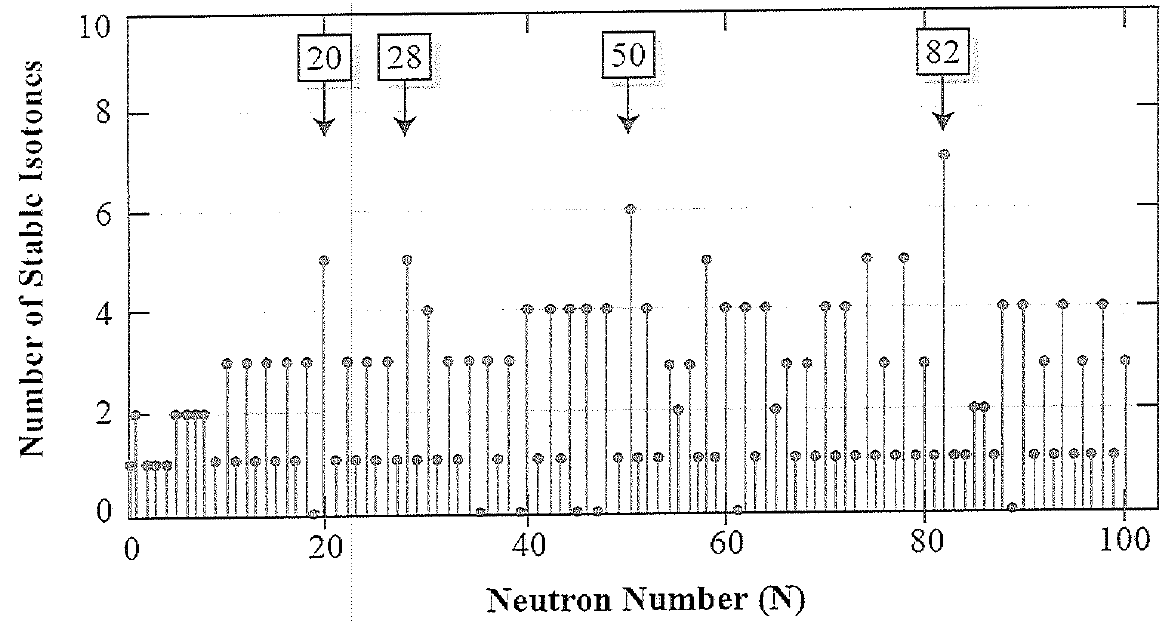
\includegraphics[width=3in]{images/shell/shell-evidence-1.png}
    \caption{Shell Model Evidence 1: Histogram of Stable Isotones Showing Nuclides with Magic Numbers Are More Abundant}
\end{figure}
\item Neutron separation energy $S_n$ is low for nuclei with one more neutron than a magic number. Reason: it is easier to separate one neutron when number of neutrons is magic plus 1; that is, magic neutron numbers are more tightly bound \footnote{Also see Krane Figure 5.2}. 
\begin{figure}[ht]
    \centering
    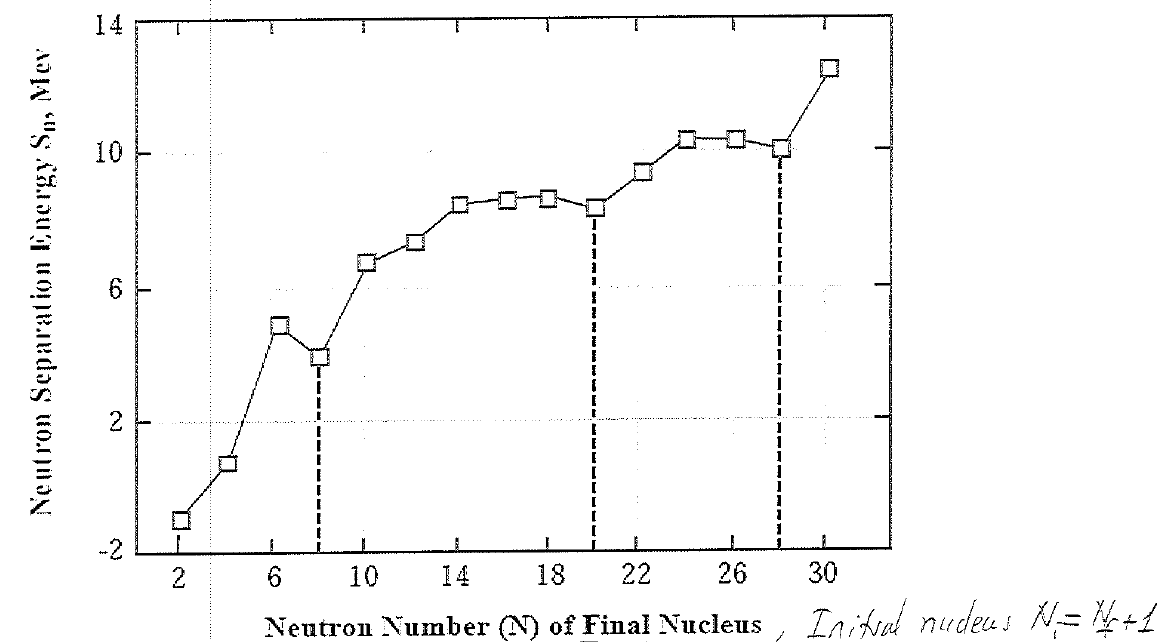
\includegraphics[width=3in]{images/shell/shell-evidence-2.png}
    \caption{Shell Model Evidence 2: Neutron Separation Energy as a Function of Neutron Number N}
\end{figure}
\item The first excited states of even-even nuclei (meaning even neutron, even proton) have higher than usual energies at magic numbers because, again, these nuclei are tightly bound. Excite states mean take one or more nuclei to a higher state to break the bound energy. If tightly bound, then excite energy increases. 
\begin{figure}
    \centering
    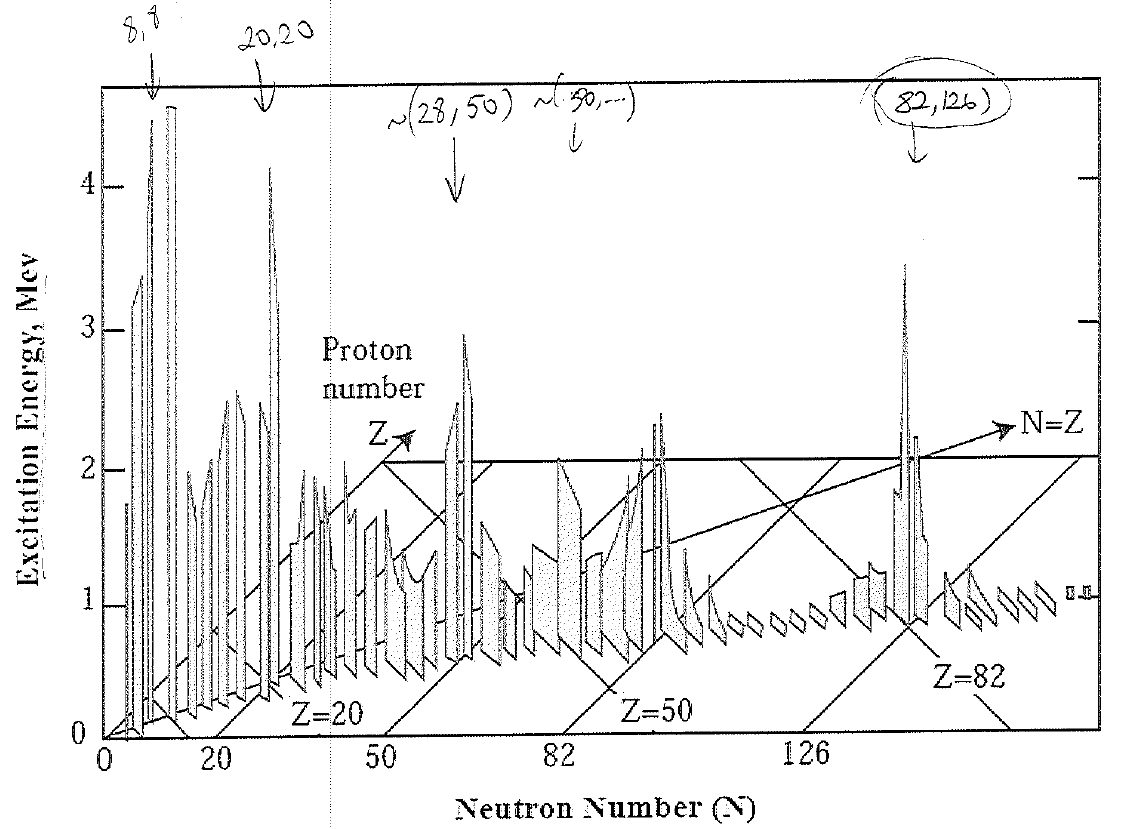
\includegraphics[width=3in]{images/shell/shell-evidence-3.png}
    \caption{Shell Model Evidence 3: First Excited States of Even-Even Nuclei Are Higher Than Usual Energies}
\end{figure}
\item Neutron capture cross sections are low for these numbers: they are stable already, do not want to absorb neutron. Zr has Z=40 and has about 50,51,52 neutrons, hence it is `neutron transparent.'
\begin{figure}
    \centering
    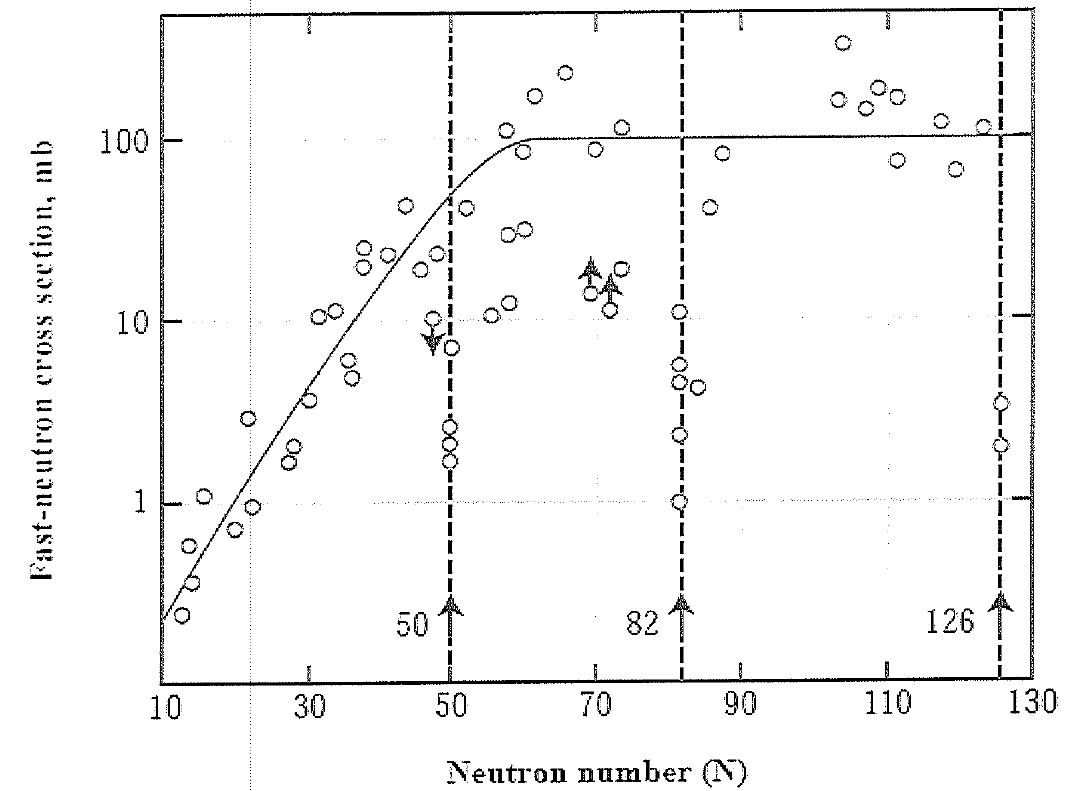
\includegraphics[width=3in]{images/shell/shell-evidence-4.png}
    \caption{Shell Model Evidence 4: Neutron Capture Cross-sections are Lower}
\end{figure}
\item Nuclear charge radius decreases and then suddenly jumps at magic numbers. 
\begin{figure}
    \centering
    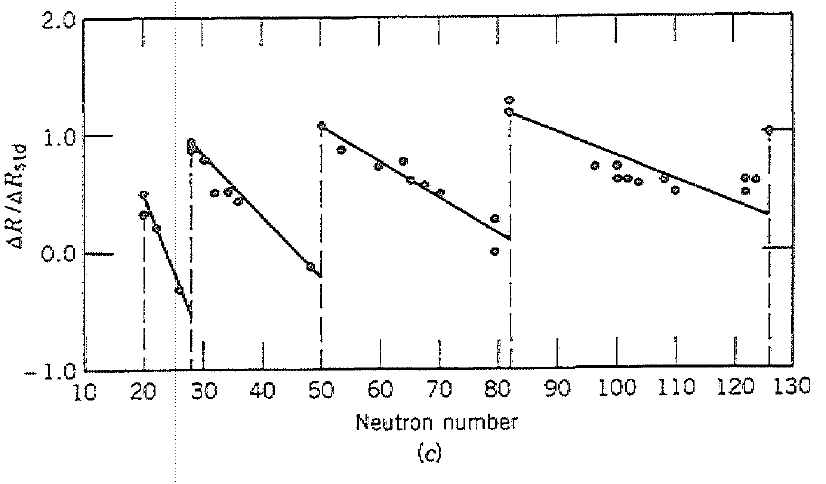
\includegraphics[width=3in]{images/shell/shell-evidence-5.png}
    \caption{Shell Model Evidence 5: Neutron Charge Radius Jumps at Magic Numbers}
\end{figure}
\end{enumerate}


\topic{Overview/Summary}
The liquid drop model leads to the SEMF, which is a smooth curve; but we know from observations, there are isotopes diverse from the smooth curve in a pattern (i.e., the nuclide with magic numbers). 


We consider the potential: The two extreme form is, when $R \to 0$ we get a harmonic oscillator potential, and when $a \to 0$ we get a square well. The real potential is somewhere between the two models. That's why we need the intermediate potential model. 


To capture the magic numbers, we consider the orbital-spin coupling. $I = j_i$ where $i$ is the singlet of the last nucleon. $j_i = l_i + s_i = l\pm \frac{1}{2}$, that is, we get degeneracy.  We can either consider the modified potential $V_{so} \to V_{so} (l \cdot s)$  or we can consider the modified energy: 
\eqn{ E_{j_i = l_i + 1/2} - E_{j_i = l_i - 1/2} = \expect{ \frac{ \left( l_i + \frac{1}{2} \right) \left( l_i + \frac{3}{2} \right) - \left( l_i - \frac{1}{2} \right) \left( l_i + \frac{1}{2} \right) }{2} V_{so} (r) } = \left( l_i + \frac{1}{2} \right) V_{so} (r) < 0  }
If we ad the spin orbit dependence onto the intermediate form, we get a form close to observations. 



\topic{Many-Body Hamiltonian} 
We are going to make the ``independent particle assumptions" which enable us to replace an n-body problem with n single-body problem:
\eqn{ \Hhat \approx \Sum_i \Hhat_i }
The independent particle assumption comes from ignoring the residual interaction terms: 
\begin{align}
 \Hhat &= \overbrace{\Sum_i \frac{\phat^2_i}{2m_i}}^{\mathrm{KE}} + \overbrace{\Sum_{i \le j} V(|x_i - x_j|)}^{\mathrm{Strong \fsp Force}} + \overbrace{\Sum_{i \le j} \frac{e^2}{|x_i - x_j|}}^{\mathrm{Coulomb, \fsp for \fsp p \fsp only}} \\
 &= \underbrace{ \Sum_i \left[ \frac{\phat^2_i}{2m_i} + V_{\mathrm{nuc}} (|x_i|) + V_{\mathrm{Coul}} (|x_i|)  \right]}_{\mbox{mean field}}  + \underbrace{\Sum_{i \le j} V(|x_i - x_j|) - \Sum V_{\mathrm{nuc}} (|x_i|) + \Sum V_{\mathrm{Coul}} (|x_i - x_j|) - \Sum V_{\mathrm{Coul}} (|x_i|) }_{\mbox{residual interactions from inter-nucleon couplings} } \\
 &= \Sum_i \Hhat_i + \underbrace{\Hhat_{\mbox{residual interaction}}}_{\to 0} \approx \Sum_i \Hhat_i \\
\Hhat_i &= \frac{\phat^2_i}{2m_i} + V_{\mathrm{nuc}} (|x_i|) + V_{\mathrm{Coul}} (|x_i|) 
\end{align}
Implications from the above derivation:
\begin{itemize}
\item Gaussian unit is used (so no $\frac{1}{4 \pi \epsilon}$ anymore); 
\item This assumption is for a independent particle single nucleon (n or p) moving in a force field ( nuclear plus coulomb) that is generated by all other nucleons; 
\item While there is strong interactions between nucleons, motion of each nucleon is practically independent of any other nucleon; 
\item $V_{\mathrm{Coul}} (|x_i|)$ term exists for protons only; 
\item Potential terms ($V_{\mathrm{nuc}} (|x_i|), V_{\mathrm{Coul}} (|x_i|)$) need to be modeled; choice of potential is important in predictions (see next section).
\end{itemize}

To model the potential, we will consider the following common ones: 
\begin{enumerate}
\item Infinite Well. It does not work because it requires infinite amount of energy to separate a $n$ or $p$; model has sharp edge, whereas nuclear charge and matter distribution fall smoothly to zero beyond the mean radius.
\item Harmonic Oscillator: the potential is parabolic. It does not work because the energy goes to infinity, and the potential inside of the well is not sharp enough (compare with experimental results); its advantage is that it allows analytical solution;
\item Intermediate Potential: somewhat like a finite potential well (has a region of -$V_0$), but the edge is smooth. 
\end{enumerate}

%%%%%%%%%%%%%%% Harmonic Oscillator %%%%%%%%%%%%
\topic{Harmonic Oscillator Potential Model}


\subtopic{Derive Potentials}
We define the potential well as a parabolic well from $-R_0$ to $R_0$ with a maximum depth of $-V_0$: 
\begin{align}
V_{\mathrm{nuc}} (r) &\approx - V_0 \left( 1 - \frac{r^2}{R_0^2} \right) = \frac{V_0}{R_0^2} (r^2 - R_0^2)  \\
V_{\mathrm{Coul}} (r) &= \frac{(Z-1) e^2}{R_0} \left[ \frac{3}{2} - \frac{1}{2}  \frac{r^2}{R_0^2}\right] 
\end{align}
Notice, again, $V_{\mathrm{Coul}}$ is only a concern for the protons; for constant proton density inside the nucleus, coulomb field is parabolic, though as $r > R_0$, real coulomb potential remains positive (and small), while the parabolic model goes to negative: 

\begin{figure}[h!]
    \centering
    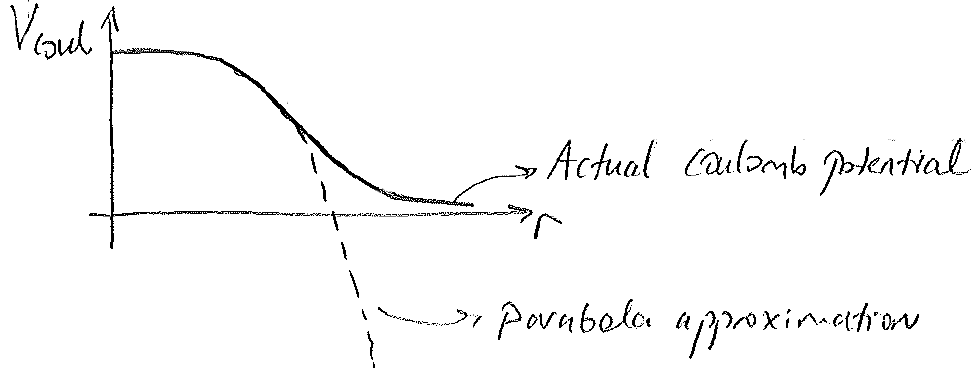
\includegraphics[width=3in]{images/shell/Vcoul-parabolic-model.png}
    \caption{Actual Coulomb Potential vs. Its Parabolic Approximation}
\end{figure}

\begin{align}
V_{\mathrm{eff}} (r) = 
\begin{dcases*}
V_{\mathrm{nuc}}  = \frac{V_0}{R_0^2} r^2 - V_0 
& neutrons (deeper,narrower well) \\
V_{\mathrm{nuc}} + V_{\mathrm{Coul}} = \overbrace{ r^2 \left[ \frac{V_0}{R_0^2} - \frac{(Z_1)e^2}{2 R_0^3} \right] }^{\frac{1}{2} m \omega^2 r^2} - \overbrace{ \left[  V_0 - \frac{3}{2} \frac{(Z-1) e^2}{R_0} \right] }^{V_0^{\prime} }   & protons (shallower,wider well) 
\end{dcases*}
\end{align}

From the above discussion, we can see that $V_{\mathrm{eff}}$ takes the general form of $\boxed{V_{\mathrm{eff}} = \frac{1}{2} m \omega^2 r^2 - V_0^{\prime}},$ 
\begin{align}
\omega^2 =
\begin{dcases*}
\frac{2}{m} \frac{V_0}{R_0^2}  & neutrons \\
\frac{2}{m} \left[ \frac{V_0}{R_0^2} - \frac{(Z-1) e^2}{2 R_0^3} \right] & protons \\
\end{dcases*}
\fsp \fsp \fsp \fsp \fsp
V_0^{\prime} = 
\begin{dcases*}
V_0 & neutrons \\
V_0 - \frac{3}{2} \frac{(Z-1) e^2}{R_0} & protons \\
\end{dcases*}
\end{align}


\end{document}
